% !TEX root = ../popl-paper.tex

\begin{figure}[ht]
	\begin{center}
		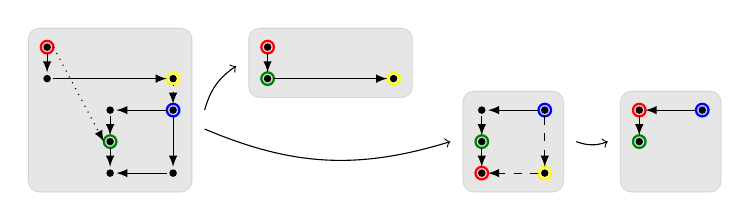
\begin{tikzpicture}[scale = .8]
			\begin{scope}
				\draw[gray,fill = gray, rounded corners, opacity=0.2] (-.3,.3) rectangle (2.3,-2.3);
				\draw[red, thick, fill = red!20] (0,0) circle (0.1);
				\draw[Green, thick, fill = Green!20] (1,-1.5) circle (0.1);
				\draw[Yellow, thick, fill = Yellow!20] (2,-.5) circle (0.1);
				\draw[blue, thick, fill = blue!20] (2,-1) circle (0.1);

				\draw[black, fill = black] (0,0) circle (.05);
				\draw[black, fill = black] (0,-.5) circle (.05);
				\draw[black, fill = black] (2,-.5) circle (.05);
				\draw[black, fill = black] (1,-1) circle (.05);
				\draw[black, fill = black] (2,-1) circle (.05);
				\draw[black, fill = black] (1,-1.5) circle (.05);
				\draw[black, fill = black] (1,-2) circle (.05);
				\draw[black, fill = black] (2,-2) circle (.05);

				\draw[>=latex, ->] (0,-.1) to (0, -.4);
				\draw[>=latex, dotted, ->] (.1,0) to (.9, -1.5);
				\draw[>=latex, ->] (.1,-.5) to (1.9, -.5);
				\draw[>=latex, dotted, ->] (2,-.6) to (2, -.9);
				\draw[>=latex, ->] (1.9,-1) to (1.1, -1);
				\draw[>=latex, ->] (1,-1.1) to (1, -1.4);
				\draw[>=latex, ->] (1,-1.6) to (1, -1.9);
				\draw[>=latex, ->] (2,-1.1) to (2, -1.9);
				\draw[>=latex, ->] (1.9,-2) to (1.1, -2);

				\draw[->] (2.5,-1) to[bend left = 20] (3,-.3);
				\draw[->] (2.5,-1.3) to[bend right = 20] (6.4,-1.5);
				\draw[->] (8.4,-1.5) to[bend right = 20] (8.9,-1.5);


			\end{scope}
			\begin{scope}[shift = {(3.5,0)}]
				\draw[gray,fill = gray, rounded corners, opacity=0.2] (-.3,.3) rectangle (2.3,-.8);
				\draw[red, thick, fill = red!20] (0,0) circle (0.1);
				\draw[Green, thick, fill = Green!20] (0,-.5) circle (0.1);
				\draw[Yellow, thick, fill = Yellow!20] (2,-.5) circle (0.1);

				\draw[black, fill = black] (0,0) circle (.05);
				\draw[black, fill = black] (0,-.5) circle (.05);
				\draw[black, fill = black] (2,-.5) circle (.05);

				\draw[>=latex, ->] (0,-.1) to (0, -.4);
				\draw[>=latex, ->] (.1,-.5) to (1.9, -.5);
			\end{scope}
			\begin{scope}[shift = {(5.9,0)}]
				\draw[gray,fill = gray, rounded corners, opacity=0.2] (.7,-.7) rectangle (2.3,-2.3);
				\draw[red, thick, fill = red!20] (1,-2) circle (0.1);
				\draw[Green, thick, fill = Green!20] (1,-1.5) circle (0.1);
				\draw[Yellow, thick, fill = Yellow!20] (2,-2) circle (0.1);
				\draw[blue, thick, fill = blue!20] (2,-1) circle (0.1);

				\draw[black, fill = black] (1,-1) circle (.05);
				\draw[black, fill = black] (2,-1) circle (.05);
				\draw[black, fill = black] (1,-1.5) circle (.05);
				\draw[black, fill = black] (1,-2) circle (.05);
				\draw[black, fill = black] (2,-2) circle (.05);
				\draw[>=latex, ->] (1.9,-1) to (1.1, -1);
				\draw[>=latex, ->] (1,-1.1) to (1, -1.4);
				\draw[>=latex, dashed, ->] (1,-1.6) to (1, -1.9);
				\draw[>=latex, dashed, ->] (2,-1.1) to (2, -1.9);
				\draw[>=latex, dashed, ->] (1.9,-2) to (1.1, -2);
			\end{scope}

			\begin{scope}[shift = {(8.4,0)}]
				\draw[gray,fill = gray, rounded corners, opacity=0.2] (.7,-.7) rectangle (2.3,-2.3);
				\draw[red, thick, fill = red!20] (1,-1) circle (0.1);
				\draw[Green, thick, fill = Green!20] (1,-1.5) circle (0.1);
				%\draw[Yellow, thick, fill = Yellow!20] (2,-2) circle (0.1);
				\draw[blue, thick, fill = blue!20] (2,-1) circle (0.1);

				\draw[black, fill = black] (1,-1) circle (.05);
				\draw[black, fill = black] (2,-1) circle (.05);
				\draw[black, fill = black] (1,-1.5) circle (.05);

				\draw[>=latex, ->] (1.9,-1) to (1.1, -1);
				\draw[>=latex, ->] (1,-1.1) to (1, -1.4);
				\end{scope}

		\end{tikzpicture}
	\end{center}
  \caption{Decomposition game for the MSC of Fig.~\ref{fig:pp_ex}. This is a 3-winning game for Eve.}
  \label{fig:stw-ex}
\end{figure}
